\documentclass[a4paper, 12pt]{article}
\usepackage{barinov}
\begin{document}
\thispagestyle{empty}
\begin{center}
    \textit{Федеральное государственное автономное образовательное\\ учреждение высшего образования }

    \vspace{0.5ex}

        \textbf{«Московский физико-технический институт\\ (национальный исследовательский университет)»}
\end{center}

\vspace{10ex}

\begin{center}
    \vspace{13ex}

    \so{\textbf{Лабораторная работа №-.-.-}}

    \vspace{1ex}

    по курсу общей физики

    на тему:

    \textbf{\textit{<<>>}}

    \vspace{30ex}

    \begin{flushright}
        \noindent
        \textit{Работу выполнил:}\\  
        \textit{Баринов Леонид \\(группа Б02-827)}
    \end{flushright}
    \vfill
    Долгопрудный \\2019
\newpage
\setcounter{page}{1}
\fancyhead[R]{\nouppercase{\leftmark}}	
\end{center}

\section{Аннотация}
В работе будут изучены оптические методы измерения углов и методы
измерения показателя преломления. Также будет проведено измерение
дисперсии света с помощью гониометра-спектрометра ГС-2.

\section{Теоретические сведения}
\subsubsection*{Преломление света в призме}
\textit{Спектральной призмой} называется многогранник, изготовленный
из прозрачного вещества с большой дисперсией показателя преломления
$(dn/d\lambda)$.

\begin{figure}[H]
    \includegraphics[width=0.6\linewidth]{1} 
    \caption{Ход лучей в призме в ее главном сечении}
    \label{fig:1}
\end{figure}

\textit{Главным сечением} называется любая плоскость, перпендикулярная
ребрам двугранных углов (\fig{fig:1}). Рассмотрим преломление призмой
пучка света в плоскости, перпендикулярной ребрам призмы
(\textit{плоскости главного сечения}). 

Из геометрического рассмотрения и закона преломления можно получить
систему уравнений для $i_1',\ i_2',\ i_2$ и $\phi$ ($\alpha,\ n$ и
$i_1$ обычно заданы):

\begin{equation}
    \left\{
       \begin{gathered}
           \sin i_1 = n \sin i_1' \\
           n\sin i_2 = \sin i_2' \\
           \phi = i_1 + i_2' - \alpha \\
           \alpha = i_1'+i_2
       \end{gathered}
    \right.
    \label{eq:1}
\end{equation}
Угол отклонения $\phi$ зависит от угла падения пучка на призму $i_1$ и
при некотором значении этого угла имеет минимум.

Дифференцируя уравнение для $\phi$ в системе уравнений \eqref{eq:1},
найдем условие минимума отклонения
\begin{equation*}
    \begin{aligned}
        d\phi/di_1 = di_2'/di_1 - 1 = 0 \\
        di_2'/di_1 = 1\quad \text{или}\quad i_1 = i_2'
    \end{aligned}
\end{equation*}
Поскольку $\alpha = -i_1'+i_2$ и $i_1' < 0$, то
\[
    \alpha = 2i_2\quad \text{или}\quad i_1' = i_2 = \alpha/2
\]
Для угла отклонения $\phi = -i_1 + i_2' - \alpha$ при $i_1 < 0$ получим
\begin{equation}
    \phi_\text{min} = 2i_1 - \alpha
    \label{eq:2}
\end{equation}
Таким образом, минимальному значению $\phi$ соответствует симметричное
прохождения пучка, при котором $i_1=i_2=i_0$ и соответственно
$i_1'=i_2'=i_0' = \alpha/2$.

В условиях минимального отклонения из соотношений, представленных выше
получим
\begin{equation}
    n = \frac{\sin \left[(\phi_\text{min} + \alpha)/2
    \right]}{\sin(\alpha/2)}
    \label{eq:3}
\end{equation}

\subsubsection*{Угловая дисперсия призмы}
Угловой дисперсий призмы называется отношение $d\phi/d\lambda$.
Дифференцируя все выражения в системе \eqref{eq:1} по $i_2$, получим
для угловой дисперсии
\begin{equation}
    \frac{d\phi}{d\lambda} = \frac{\sin\alpha}{\cos i_1' \cdot \cos
    i_2'} \cdot \frac{dn}{d\lambda}
    \label{eq:4}
\end{equation}

Если призма установлена у условиях минимального отклонения $i_1=i_2 =
i_0$ и $i_1'=i_2'=\alpha/2$, то выражение \eqref{eq:4} можно записать
в виде
\begin{gather}
    \frac{d\phi}{d\lambda} = 2 \frac{\sin i_0'}{\sin i_0} \cdot
    \frac{dn}{d\lambda} =
    \frac{2\sin\alpha/2}{\sqrt{1-n^2\sin\alpha/2}}\cdot
    \frac{dn}{d\lambda} 
    \label{eq:5} \\
    \frac{d\phi}{d\lambda} = \frac{2}{n} \tg\alpha \frac{dn}{d\lambda}
    = \frac{D}{t} \cdot \frac{dn}{d\lambda} \label{eq:6}
\end{gather}
Здесь $D$ --- ширина падающего пучка, $t$ --- длина основания призмы,
заполненной светом (или разность длин путей в призме двух крайних
лучей пучка в плоскости главного сечения).


\section{Оборудование}
\textbf{В работе используются:} гониометр ГС-2, спектральные призмы.

Конструкция гониометра ГС-2. На массивном основании гониометра
\textsl{14} установлен коллиматор \textsl{11}, а внутри помещена
осевая система (\textsl{рис. 2.20}). На массивной оси системы закреплена
вращающая алидада \textsl{13} с закрепленной на ней зрительной трубой
\textsl{2}. На конце этой же оси закреплен предметный столик
\textsl{6}. Внутри корпуса алидады смонтирована оптическая система для
снятия отсчета с лимба и механизмы точного вращения алидады и лимбы

\begin{figure}[H]
    \includegraphics[width=\linewidth]{2} 
    \label{fig:2}
\end{figure}
\begin{figure}[H]
    \includegraphics[width=0.59\linewidth]{3} 
    \label{fig:3}
\end{figure}

\section{Результаты измерений и обработка результатов}
\subsubsection*{Измерение преломляющего угла призмы}

\begin{wrapfigure}{r}{0.5\linewidth}
    \vspace{-10pt}
    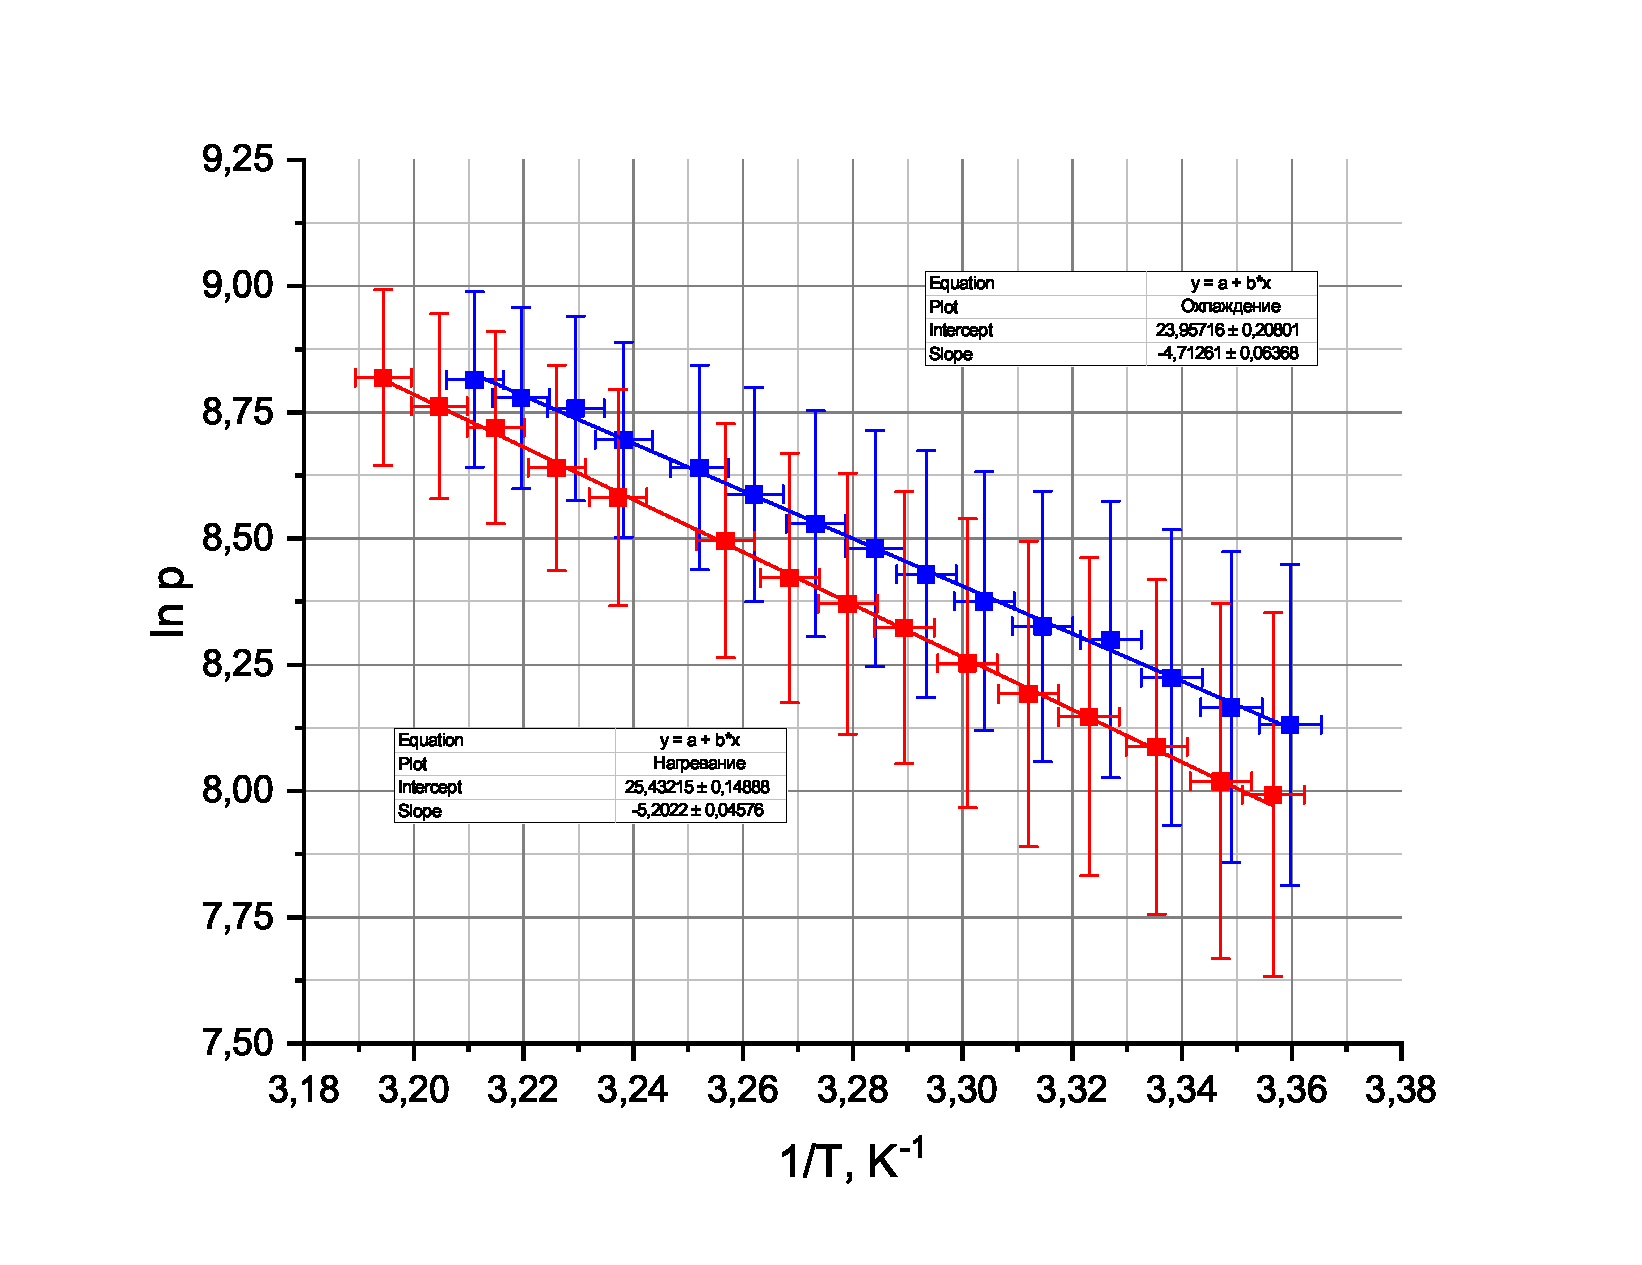
\includegraphics[width=\linewidth]{4}
    \caption{Схема измерения двугранного угла призмы. $M$ --- призма,
    AK --- автоколлимационная труба}
    \label{fig:4}
\end{wrapfigure}

Схема измерения угла между гранями призмы автоколлимационным способом
показана на \fig{fig:4}. Вращением столика с лимбом сначала грубо от
руки, а затем с помощью механизма точно наводки совмещаем
автоколлимационное изображение вертикального штриха с вертикальным
штрихом сетки окуляра. Это операция называется
\textit{автоколлимационным наведением}. Снимем отсчет $N_1$ положения
алидады по отсчетному устройству. Проведем автоколлимационное
наведение на вторую грань призмы и снимем отсчет $N_2$. Значение угла
между гранями:
\[
    \alpha = 180^\circ - \vartheta
\]
где $\vartheta = N_1 - N_2$
\[
    \alpha = 180^\circ - (160^\circ48'55'' - 43^\circ46'32'') =
    62^\circ 57' 37''
\]

\subsubsection*{Измерение показателя преломления стекла методом угла
наименьшего отклонения (метод Фраунгофера)}

\begin{wrapfigure}{l}{0.5\linewidth}
    \includegraphics[width=\linewidth]{5}
    \caption{Схема измерения показателя преломления методом угла
    наименьшего отклонения. $M$ --- призма, $K$ --- коллиматор, $AK$
--- автоколлимационная труба}
\label{fig:5}
\end{wrapfigure}

В основе метода лежит зависимость \eqref{eq:2} между углом
минимального отклонения $\phi$, преломляющим углом призмы $\alpha$ и
показателем преломления $n$:
\[
    n = \frac{\sin[(\phi_\text{min}+\alpha)/2]}{\sin(\alpha/2)}
\]

Схема измерения показателя преломления $n$ методом наименьшего угла
отклонения показана на \fig{fig:5}.

Щель коллиматора освещается спектральной лампой, дающей набор
монохроматических линий излучения. Изображения цели коллиматора,
преломленные призмой, рассматриваются в окуляр зрительной трубы.

Поворачивая столик с призмой и алидаду со зрительной трубой так, чтобы
изображение щели коллиматора оставалось в поле зрения, найдем такое
положение столика, при котором отклонение для выбранной спектральной
линии будет минимальным. Зафиксируем столик относительно оси
гониометра зажимным винтом. Совместим изображение щели с вертикальным
штрихом сетка окуляра и снимем отсчет $N_1$.

Затем, не изменяя положение столика, повернем алидаду и совместим
неотклоненное призмой изображение щели с вертикальным штрихом сетки
окуляра. Снимем отсчет $N_2$. Наименьший угол отклонения равен
\[
    \phi_\text{min} = N_1 - N_2
\]

В качестве источника света используется лампа ДРС-50 ($Hg$). Спектр
этой лампы приведен на \fig{fig:6}


\begin{figure}[H]
    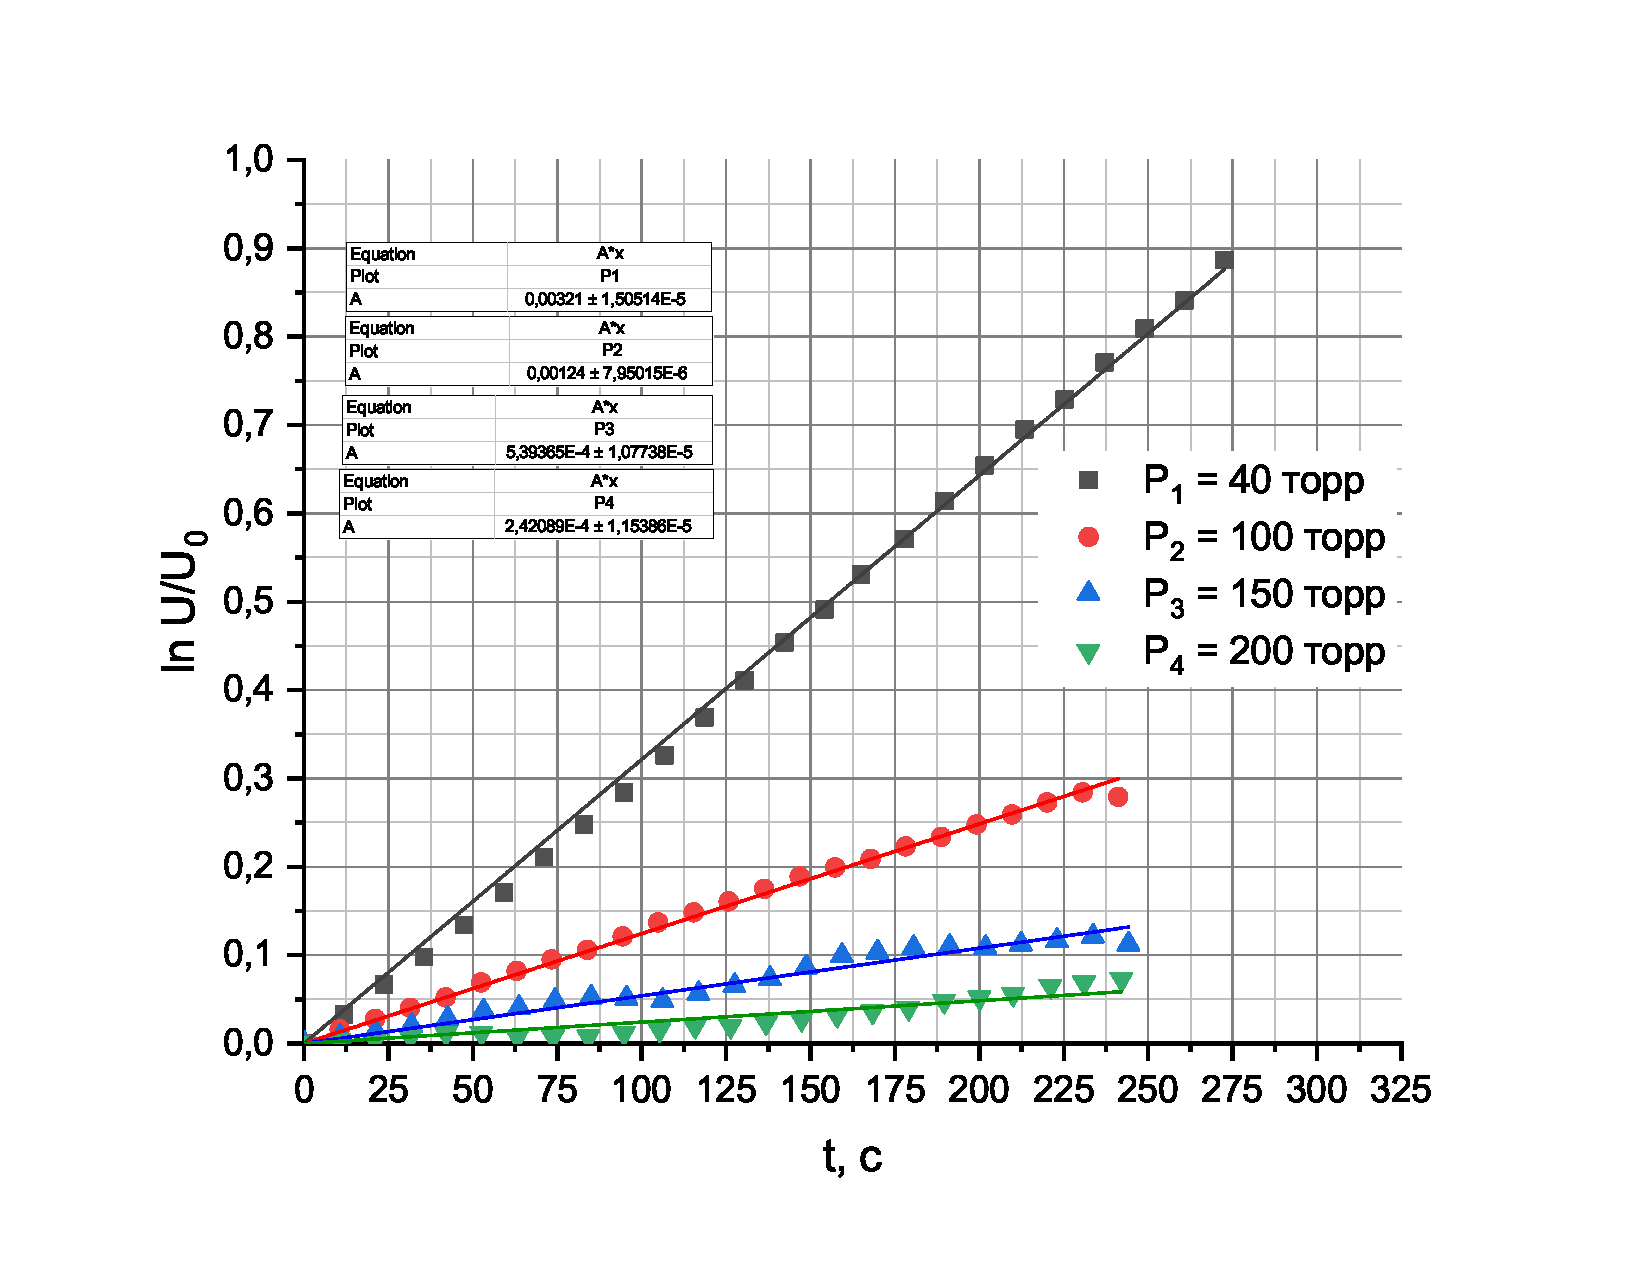
\includegraphics[width=0.8\linewidth]{6} 
    \caption{Спектры излучения ртутной лампы ДРС-50. Значения длин
    волн линий приведены в нм}
    \label{fig:6}
\end{figure}

\[
    N_1 = 160^\circ 11' 57''
\]

Снимем значения $N_2$: желтая левая полоска --- $212^\circ 42'37''$,
желтая правая полоска --- $212^\circ 42' 19''$, зеленая полоска ---
$213^\circ 5' 28''$, фиолетовая полоска --- $215^\circ 22' 52''$,
синяя левая полоска --- $213^\circ 58' 30''$, синяя правая полоска ---
$213^\circ 53' 30''$, голубая полоска --- $213^\circ 44' 55''$. По
формуле для $\phi_\text{min}$ и по формуле \eqref{eq:3} вычислим
значения показателя преломления $n$.

\renewcommand{\arraystretch}{1.2}
\begin{table}[H]
\centering
\begin{tabular}{|c|c|}
    \hline 
    $\lambda,\ \text{нм}$ & $n$ \\ \hline 
 579 & 1.61928 \\ \hline 
 586 & 1.61924 \\ \hline 
 546.07 & 1.62267 \\ \hline 
 435 & 1.64267 \\ \hline 
 491.61 & 1.63047 \\ \hline 
 497.36 & 1.62974 \\ \hline 
 503 & 1.62848 \\ \hline 
\end{tabular}
\caption{Зависимость значения показателя преломления $n$ от длины
волны $\lambda$}
\end{table}

Построим график зависимости $n(\lambda)$:

\begin{figure}[H]
    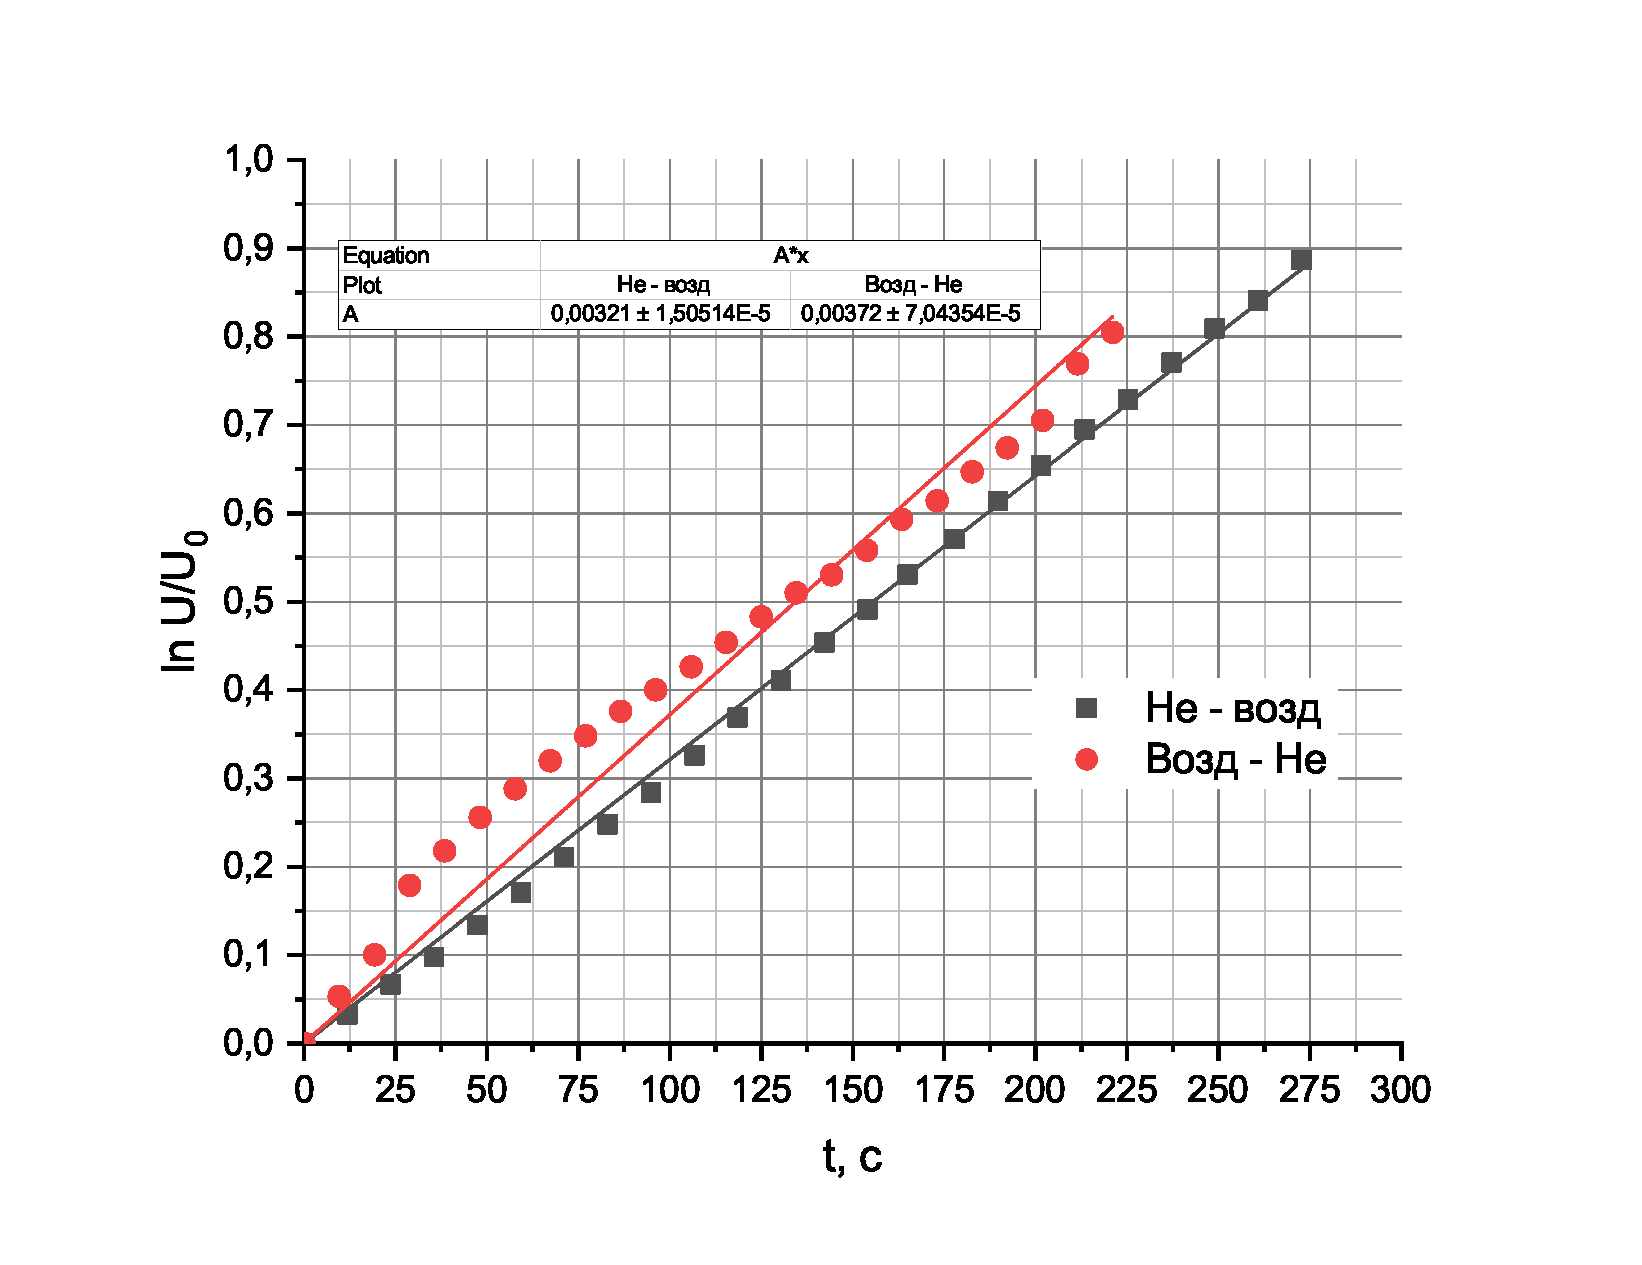
\includegraphics[width=\linewidth]{8} 
    \caption{График зависимости значения показателя преломления $n$ от длины
волны~$\lambda$}  
\label{fig:8}
\end{figure}

\subsubsection*{Измерение зависимости угловой дисперсии призмы от угла
падения луча на призму}

Изучение зависимости угловой дисперсии призмы от угла падения
производится путем измерения угла $\Delta \phi$ между изображениями
двух близких спектральных линий с известной разницей длин волна
$\Delta \lambda$:
\[
    \frac{d\phi}{d\lambda} \approx \frac{\Delta \phi}{\Delta \lambda}
\]
при различных углах $i_1$ падения лучей на призму

Схема измерения показана на \fig{fig:7}.


\begin{figure}[H]
    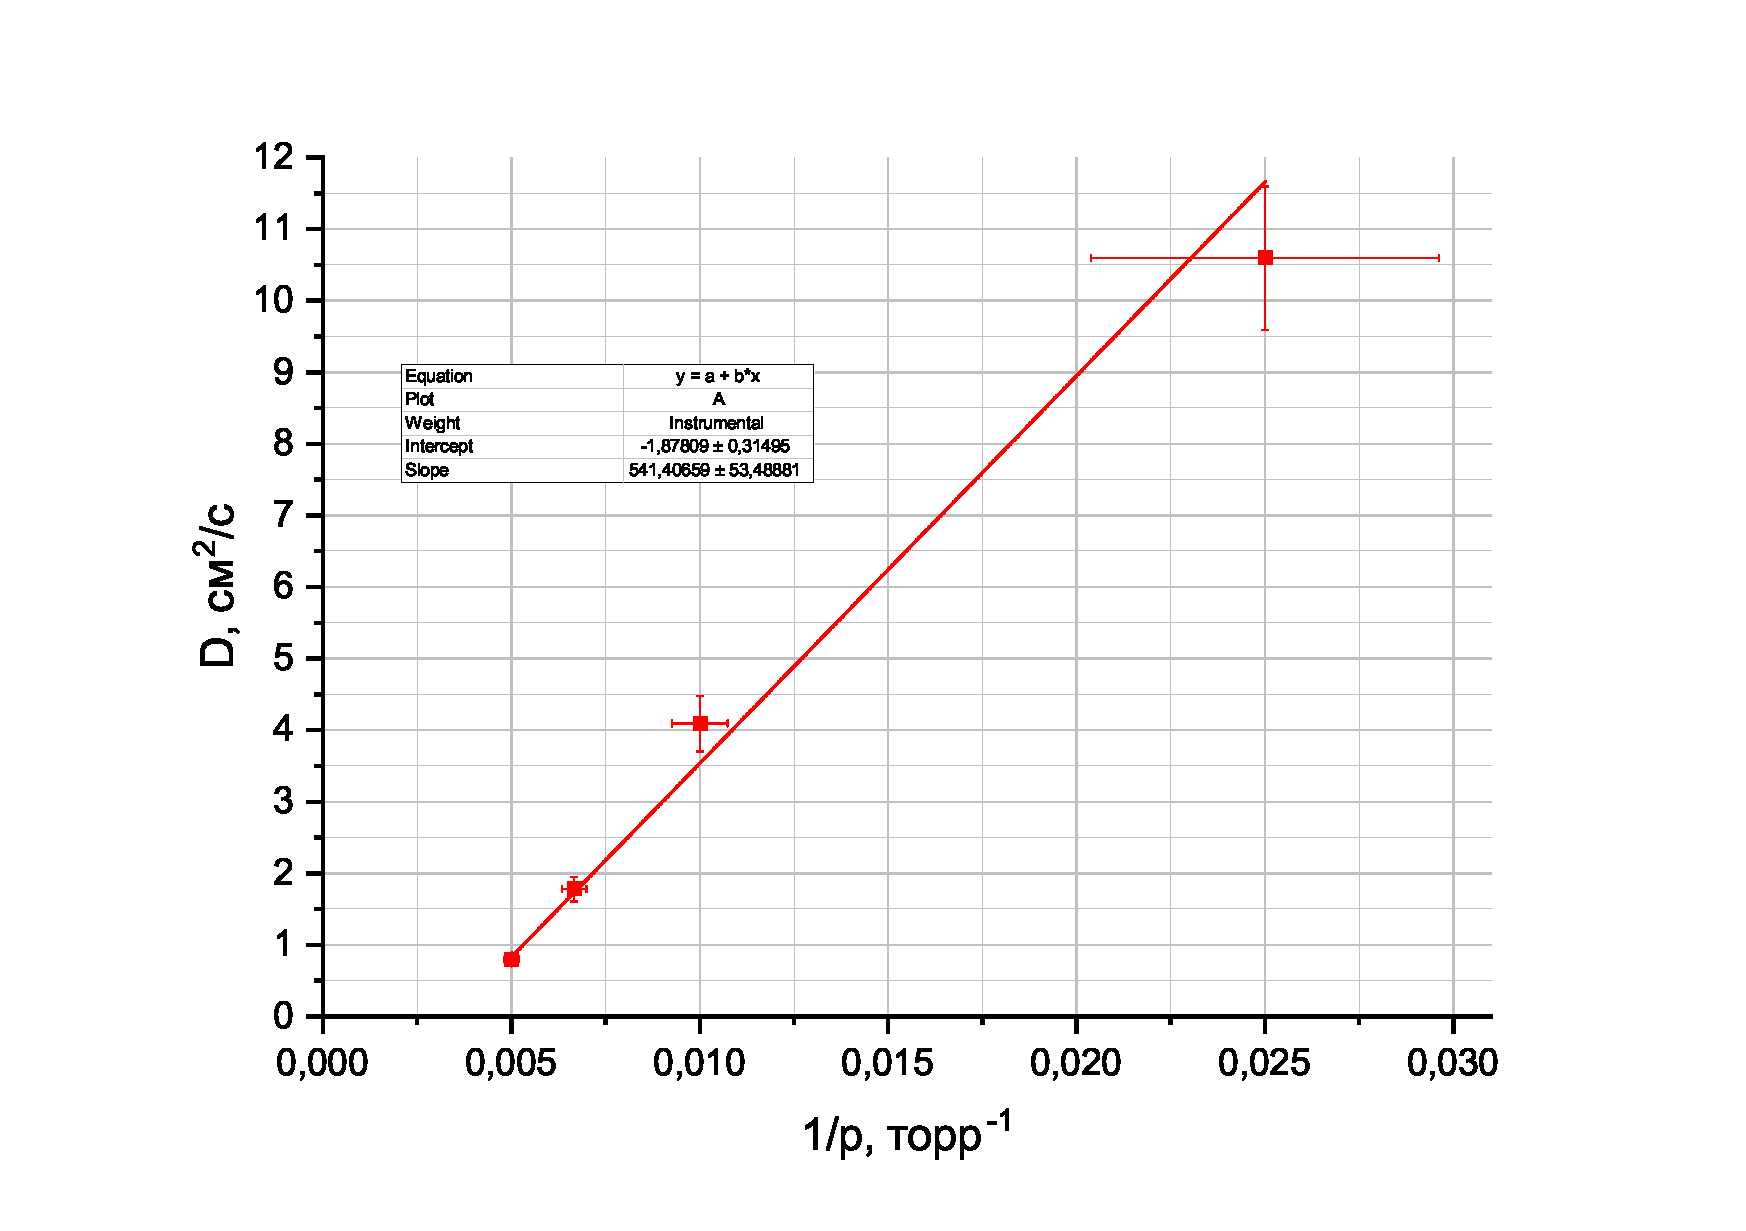
\includegraphics[width=0.6\linewidth]{7} 
    \caption{Схема измерения зависимости угловой дисперсии призмы
    $d\phi/d\lambda$ от угла падения света на призму $i_1$. $M$ ---
призма, $K$ --- коллиматор, $AK$ --- автоколлимационная труба}
\label{fig:7}
\end{figure}

Совместим изображение цели на длине волны $\lambda_1$ с вертикальным
штрихом сетки окуляра зрительной трубы и запишем отсчет $N_1$. Затем
совместим изображение цели на длине волны $\lambda_2$ и запишем отсчет
$N_2$. Значение угла $\Delta \phi$ равно
\[
    \Delta \phi = N_1-N_2
\]
а величина угловой дисперсии 
\[
    \frac{d\phi}{d\lambda} \approx \frac{\Delta \phi}{\Delta \lambda}
    = \frac{N_1 - N_2}{\lambda_1 - \lambda_2}
\]
где угол $\Delta \phi$ выражен в радианах.

Измерим угол падения света на преломляющую грань призмы $i_1$. Для
этого повернем алидаду и проведем автоколлимационное наведение на
грань призмы. Снимем отсчет $N_3$. Повернем алидаду и совместим не
преломленное призмой изображение щели с вертикальным штрихом сетки
окуляра зрительной трубы. Снимем отсчет $N_4$. Угол падения лучей на
призму $i_1 = \alpha - \theta$, где $\theta = N_3 - N_4$.


\begin{table}[H]
\centering
\begin{tabular}{|c|c|c|c|c|c|}
\hline
$N_1,\ ^\circ$        & $N_2,\ ^\circ$        & $N_3,\ ^\circ$
                      & $N_4,\ ^\circ$        & $i,\ ^\circ$        &
                      \specialcell{$d\phi/d\lambda,$ \\ $10^3\
                      \text{м}^{-1}  $}\\ \hline
213,010 & 212,902 & 148,740 & 160,217 & 74,437 & 894,599  \\ \hline
215,417 & 215,217 & 142,050 & 160,217 & 81,127 & 1662,222 \\ \hline
212,848 & 212,757 & 150,723 & 160,217 & 72,454 & 759,543  \\ \hline
219,056 & 218,889 & 142,058 & 160,217 & 81,119 & 1385,185 \\ \hline
212,397 & 212,373 & 156,437 & 160,217 & 66,740 & 195,080  \\ \hline
\end{tabular}
\caption{Зависимость угловой дисперсии $d\phi/d\lambda$ от угла
падения $i_1$}
\end{table}

\begin{figure}[H]
    \includegraphics[width=\linewidth]{9} 
    \caption{График зависимости угловой дисперсии $d\phi/d\lambda$ от угла
падения $i_1$}
\label{fig:9}
\end{figure}


\section{Обсуждение результатов и выводы}
В работе был измерен преломляющий угол призмы $\alpha$:
\[
    \alpha = 62^\circ 57' 37''
\]

Исследована зависимость значения показателя преломления $n$ от длины
волны $\lambda$ методом Фраунгофера (\fig{fig:7}). Значения,
полученные в эксперименте хорошо согласуются с теоретической
зависимостью:
\[
    n = 1 + \frac{4\pi N q^2}{m\left(\omega_0^2 -
    \left(\dfrac{2\pi}{\lambda}\right)^2\right)}
\]

Также исследована зависимость угловой дисперсии $d\phi/d\lambda$ от
угла падения $i_1$ (\fig{fig:9}). С увеличением угла падения $i_1$
увеличивается угловая дисперсия $d\phi/d\lambda$.






\end{document}
